% !TeX root = technical-report.tex
\documentclass[10pt,a4paper]{article}
\usepackage[utf8]{inputenc}
\usepackage[T5,T1]{fontenc}
\usepackage{lmodern}
\usepackage[margin=19mm,headheight=14pt,headsep=6mm,footskip=10mm]{geometry}
\usepackage{amsmath,amssymb,graphicx,booktabs,array,tabularx}
\usepackage[table]{xcolor}
\usepackage{microtype,fancyhdr,lastpage}
\usepackage[font=small,labelfont=bf,skip=5pt]{caption}
\usepackage[hyphens]{url}
\usepackage[colorlinks=true,linkcolor=blue!45!black,citecolor=blue!45!black,urlcolor=blue!45!black]{hyperref}
\definecolor{ink}{HTML}{17324D}
\definecolor{accent}{HTML}{167D9A}
\newcommand{\reportauthor}{{\fontencoding{T5}\selectfont Kiên Nguyễn}}
\pagestyle{fancy}
\fancyhf{}
\fancyhead[L]{\small\textcolor{ink}{MiniGrid Exploration Agent}}
\fancyhead[R]{\small Atherlabs technical test}
\fancyfoot[L]{\footnotesize\textcolor{ink}{\reportauthor\ / MiniGridRL}}
\fancyfoot[R]{\footnotesize\thepage\,/\,\pageref*{LastPage}}
\renewcommand{\headrulewidth}{0.3pt}
\setlength{\parindent}{0pt}
\setlength{\parskip}{4pt plus 1pt}
\setlength{\textfloatsep}{8pt}
\setlength{\intextsep}{8pt}
\renewcommand{\arraystretch}{1.13}
\newcommand{\pct}{\%}
\newcommand{\code}[1]{\texttt{\small #1}}
\newcommand{\heading}[1]{\vspace{5pt}{\large\bfseries\color{ink}#1}\par\vspace{1pt}}
\newcommand{\subheading}[1]{\textbf{\color{ink}#1}\enspace}
% Generated from verified confirmation seeds 40000-40099.
\newcommand{\AlignedCoverage}{90.8}
\newcommand{\OriginalCoverage}{68.9}
\newcommand{\MaplessCoverage}{78.6}
\newcommand{\FrontierCoverage}{91.5}
\newcommand{\NoBonusCoverage}{59.6}
\newcommand{\PrimaryEpisodes}{5,700}
\newcommand{\TotalParameters}{649,925}
\newcommand{\MapParameters}{459,008}
\newcommand{\TranslationFlips}{13.5}
\newcommand{\RotationFlips}{20.5}
\newcommand{\RewardGains}{Easy +16.2 [13.5, 19.1]; Medium +35.8 [32.2, 39.6]; Hard +41.6 [37.8, 45.3]}

\hypersetup{pdftitle={Learning Exploration with Agent-Aligned Map Memory in MiniGrid},pdfauthor={Kiên Nguyễn},pdfsubject={Atherlabs - Reinforcement Learning Engineer Technical Test}}
\begin{document}
{\LARGE\bfseries\color{ink}Learning Exploration with\\[3pt]Agent-Aligned Map Memory in MiniGrid\par}
\vspace{5pt}
{\small\reportauthor\hfill Atherlabs --- Reinforcement Learning Engineer Technical Test\par}
\vspace{6pt}
\textbf{Abstract.} A PPO agent combines local perception with observation-derived spatial memory to explore partially observed maps, discover points of interest (POIs), and avoid a moving threat. An initial map policy underperformed mapless PPO. Centering and rotating the remembered map around the agent improved exploration without changing network capacity or rewards. Across 5,700 reserved-map episodes, aligned coverage is \AlignedCoverage\pct, versus \OriginalCoverage\pct\ with the original map, \MaplessCoverage\pct\ without map input, \NoBonusCoverage\pct\ aligned without exploration bonuses, and \FrontierCoverage\pct\ for a frontier explorer. The comparison exposes distinct tradeoffs in exploration speed, survival, and looping; earlier map exposure is disclosed separately.

\heading{1\quad Problem formulation and environment}
We model the task as a finite-horizon POMDP $(\mathcal S,\mathcal A,P,\mathcal O,\Omega,R,\rho_0,T,\gamma)$, with initial-state distribution $\rho_0$, transition kernel $P$, observation map $\Omega$, reward $R$, budget $T$, and discount $\gamma$. A sufficient simulator-and-reward state is
\[
 s_t=(G,Q,p_t,d_t,z_t,z_t^{-},t,b_t,\mathcal H_t),\qquad
 s_{t+1}\sim P(\cdot\mid s_t,a_t),\quad o_t=\Omega(s_t).
\]
Here $G$ is traversability, $Q$ the POI locations, $(p_t,d_t)$ the agent pose, and $z_t,z_t^{-}$ the current and previous monster cells; $b_t$ stores movement/contact feedback, and $\mathcal H_t$ the discovery/visit record used by the reward. These quantities define the process, not the agent's information. From observations and actions, a deterministic wrapper updates $m_t=F(m_{t-1},o_t,a_{t-1})$. The policy acts on encoded input $x_t$ for an episode of length $\tau\leq T$:
\[
 J(\theta)=\mathbb E_{\pi_\theta,P,\rho_0}\!\left[\sum_{t=0}^{\tau-1}\gamma^t r_t\right],
 \qquad a_t\sim\pi_\theta(\cdot\mid x_t).
\]
Evaluation measures coverage, discovery, and survival separately because shaped return is only a proxy for exploration.

\subheading{Map generation.} We extend \href{https://github.com/Farama-Foundation/Minigrid}{Farama Foundation's MiniGrid}~\cite{minigrid}, retaining its movement, visibility, rendering, and Gymnasium interface. A connected depth-first maze creates backtracking paths; carved rooms and extra openings add open areas and alternative routes. Revisiting similar junctions makes spatial history relevant. Connectivity and reachable POIs are checked at generation; POIs remain traversable floor tiles.
\begin{center}\small
\begin{tabular}{lrrrr}\toprule
Preset & Grid & POIs & Action budget $T$ & Monster period\\\midrule
Easy & $15\times15$ & 2 & 512 & 3 actions\\
Medium & $21\times21$ & 3 & 1,024 & 2 actions\\
Hard & $27\times27$ & 5 & 1,536 & 2 actions\\\bottomrule
\end{tabular}
\end{center}
Larger maps increase spatial demand and receive longer travel budgets; Easy's slower patrol reduces timing pressure. These preset constants were fixed before training, without calibration for equal difficulty.

\subheading{Threat dynamics.} The monster starts at least six traversable steps away and samples legal neighbors, excluding its previous cell when alternatives exist. This creates a stochastic timing obstacle without pursuit. Separate map/patrol random streams preserve seeded reproducibility. Contact after either agent movement or a scheduled monster move terminates the episode; reaching $T$ truncates it. Discovering all POIs leaves exploration running.

\heading{2\quad Observations, actions, and memory}
The action space is $\mathcal A=\{0:\mathrm{left},1:\mathrm{right},2:\mathrm{forward},3:\mathrm{wait}\}$; waiting allows a visible patrol to pass. The observable and policy-input spaces are
\[
 \begin{gathered}
 o_t=(L_t,c_t),\quad L_t\in\{0,1\}^{5\times7\times7},\quad
 c_t=(e_{d_t},u_t,w_t,k_t,1-t/T)\in[0,1]^8,\\
 x_t=(L_t,M_t,c_t),\qquad M_t=E(m_t)\in[0,1]^{7\times55\times55}.
 \end{gathered}
\]
$L_t$ one-hot encodes MiniGrid's wall-occluded view: unseen, empty, wall, POI, or monster. In $c_t$, $e_{d_t}$ is one-hot heading; $u_t,w_t,k_t$ indicate movement success, wall contact, and monster contact. Movement feedback supports odometry, while remaining time distinguishes finite-horizon situations. The constant mission is omitted.

$M_t$ stores observed cells, walls, floor, discovered POIs, occupancy counts, currently visible monsters, and the agent. Counts are scaled as $\min(n,10)/10$; old monster positions are cleared. The canvas accommodates supported maps up to $27\times27$. Memory resets each episode; hidden terrain, hidden threats/POIs, and evaluator denominators never enter $x_t$.

\newpage
\heading{3\quad Exploration reward}
Let $S_t,V_t,D_t$ denote observed floor, occupied cells, and discovered POIs after observation $o_t$. The new-information counts for transition $t$ are
\[
 \Delta S_t=|S_{t+1}\setminus S_t|,\quad
 \Delta V_t=|V_{t+1}\setminus V_t|,\quad
 \Delta D_t=|D_{t+1}\setminus D_t|.
\]
The wrapper computes
\[
 r_t=0.02\Delta S_t+0.01\Delta V_t+\Delta D_t-0.001
       -0.02w_{t+1}-k_{t+1}.
\]
Newly seen floor provides guidance before a sparse POI discovery; first occupancy rewards actual travel. Step and wall costs discourage wasted actions. Sets are initialized from $o_0$ without reward, so revisits and repeated sightings cannot earn discovery credit. No reward clipping or running reward normalization is used.

Weights were fixed heuristically. For a 236-cell Medium map, complete revelation and visitation offer about 4.7 and 2.4 reward before subtracting reset credits; three POIs offer three. The immediate death cost equals one POI, in addition to losing future rewards. This permits high discovery reward alongside death, so survival remains a separate outcome. Removing seen/visit bonuses in matched ablations tests their contribution.

\heading{4\quad Spatial memory and policy optimization}
\subheading{Map representation.} Similar-looking junctions can require different actions depending on earlier exploration. An explicit map supplies this history using reliable movement feedback. Diagnostics found correct mapping but sensitivity to coordinates: a four-cell translation changed \TranslationFlips\pct\ of greedy decisions, and joint rotation of map and heading changed \RotationFlips\pct\ across 864 states. These out-of-distribution probes suggested testing relative alignment; the subsequent retrained comparison provides stronger evidence.

The memory readout centers the agent at $(27,27)$ with forward upward. For output column $u$, row $v$, remembered position $\hat p_t$, and forward/right vectors $f_{d_t},r_{d_t}$, all channels read the same source cell:
\[
 p_{\mathrm{src}}=\hat p_t+(27-v)f_{d_t}+(u-27)r_{d_t}.
\]
Facing east, output $(27,26)$ reads one cell east and $(28,27)$ one cell south. This presents map geometry in the same frame as relative actions. Integer gathering with zero padding preserves symbols without wrapping; storage and reward bookkeeping remain start-relative.

\subheading{Actor--critic network.} Separate CNNs encode immediate geometry and the larger historical map; heading, contact, and time remain scalar features. With alignment operator $A$, the shared representation is
\[
 \phi_t=[f_L(L_t);f_M(A(M_t,d_t));c_t]\in\mathbb R^{200},\quad
 \pi_\theta(\cdot\mid x_t)=\operatorname{softmax}(g_\pi(\phi_t)),\quad V_\theta(x_t)=g_V(\phi_t).
\]
\begin{center}\small
\begin{tabularx}{\linewidth}{@{}lXr@{}}\toprule
Component & Layers & Output\\\midrule
Local CNN & $3\times3$, $5\!\to\!16\!\to\!32$, stride 1; flatten and linear & 64\\
Map CNN & $3\times3$, $7\!\to\!32\!\to\!64\!\to\!64$, stride 2; flatten and linear & 128\\
Fusion & Local + map features + 8 scalars & 200\\
Actor / critic & Separate $200\!\to\!128\!\to\!128$ MLPs; logits / value & 4 / 1\\\bottomrule
\end{tabularx}
\end{center}
CNNs/projections use ReLU; the heads use Tanh. All variants retain \TotalParameters\ parameters, including \MapParameters\ in the map encoder; alignment adds none. The original frame uses $A(M_t,d_t)=M_t$, and the no-map ablation supplies zeros. Temporal history resides in the map, not a recurrent hidden state.

\subheading{PPO update.} PPO~\cite{ppo}, implemented in Stable-Baselines3~\cite{sb3}, supports these dictionary inputs, four discrete actions, and parallel sampling. It updates the categorical policy using rollouts from $\pi_{\theta_{\rm old}}$:
\[
 \begin{aligned}
 \varrho_t(\theta)&=\frac{\pi_\theta(a_t\mid x_t)}{\pi_{\theta_{\rm old}}(a_t\mid x_t)},\\
 L_{\rm clip}(\theta)&=\mathbb E_t\!\left[\min\!\left(\varrho_t\widehat A_t,
        \operatorname{clip}(\varrho_t,1-\epsilon,1+\epsilon)\widehat A_t\right)\right].
 \end{aligned}
\]
$\widehat A_t$ is the normalized GAE advantage, $\epsilon=0.2$, and $H$ is categorical entropy. With return target $\widehat R_t=A_t^{\rm GAE}+V_{\theta_{\rm old}}(x_t)$, the minimized loss is
\[
 \mathcal L(\theta)=-L_{\rm clip}(\theta)+0.5\,\mathbb E_t[(V_\theta(x_t)-\widehat R_t)^2]
    -0.01\,\mathbb E_t[H(\pi_\theta(\cdot\mid x_t))].
\]
 Short on-policy storage also suits the large input: 4,096 observations occupy about 335 MiB; one million uncompressed observation/next-observation pairs would require about 171 GB before replay metadata.

\newpage
\heading{5\quad Training setup and baselines}
Training mixes Easy and Medium equally per reset; Hard is withheld to test extrapolation to larger maps. Training map seeds are 0--9,999. Optimization seeds 11, 22, and 33 are repeated for five conditions: full-reward original map, full-reward no map, original map without seen/visit bonuses, full-reward aligned map, and aligned map without those bonuses. No-map PPO still maintains discovery history for rewards; only its map input is zeroed.

Each run targets five million transitions, approximately 75 million across 15 runs. The aligned no-bonus runs finish 5,001,216 transitions because PPO completes rollouts. Training uses Python 3.11 and an RTX 4090. Original-map seed 33 resumed after a CUDA failure, restarting sampling; a seed-11/22 sensitivity check addresses that reference-run concern.
\begin{center}\small
\begin{tabularx}{\linewidth}{@{}lX@{}}\toprule
Setting & Value\\\midrule
Collection & 16 subprocess environments $\times$ 256 steps; 4,096 transitions/update\\
Updates & Batch 256, four epochs, learning rate $3\times10^{-4}$\\
Return estimation & Discount $\gamma=0.99$, GAE $\lambda=0.95$\\
Update controls & Clip 0.2, entropy 0.01, target KL 0.03, value coefficient 0.5, gradient norm cap 0.5\\\bottomrule
\end{tabularx}
\end{center}
Parallel collection supplies varied trajectories; minibatch reuse limits update cost. Entropy encourages training-time action diversity, while clipping, target-KL stopping, and gradient clipping constrain update size. These settings were fixed before experimentation and several differ from SB3 defaults. The scale $1/(1-\gamma)=100$ emphasizes nearer rewards without imposing a hard planning horizon; its role in long-episode stalls has not been isolated.

CPU validation runs every 250,000 transitions on Easy/Medium seeds 10,000--10,049. Coverage AUC selects for both early discovery and sustained coverage; POI fraction and survival break ties. Selected full-reward aligned steps are 3.25M / 4.50M / 3.75M for seeds 11 / 22 / 33; aligned no-bonus steps are 3.25M / 5.00M / 2.25M. Their mean selected validation AUCs are 0.883 and 0.667 respectively. No test outcome determines checkpoint selection.

\subheading{Reference agents.} Seeded uniform random actions establish an exploration floor. The deterministic frontier baseline uses breadth-first search (BFS) through known traversable cells to reach the nearest cell bordering unexplored space, with fixed tie-breaking and visible-threat avoidance. It receives the same observation-derived map and budgets as PPO, not the hidden layout. It is a strong reference, not an upper bound. The no-map ablation changes available information and effective learning capacity because the retained map branch receives zeros.

\heading{6\quad Evaluation protocol}
The primary comparison reserves \textbf{seeds 40,000--40,099} before the new ablation training and evaluation. Its protocol freezes settings and existing model hashes; selected new checkpoint hashes are frozen before testing. An audit found no reserved seeds in 21,165 recorded episode rows, though unrecorded external use cannot be audited. No checkpoint or parameter was selected using confirmation outcomes.

\textbf{Earlier exposure.} Seeds 20,000--20,099 informed diagnosis; an earlier review also used original/mapless policies on 30,000--30,029. The archived 30,000--30,099 comparison was therefore not wholly independent confirmation. Its 70-map exclusion sensitivity remains historical evidence; the current tables use only the new reserved set.

Each PPO condition contributes $3\times100\times3=900$ episodes; random contributes 900 across three policy seeds and frontier 300, totaling \PrimaryEpisodes. PPO evaluation is greedy, $a_t=\arg\max_a\pi_\theta(a\mid x_t)$, and frontier is deterministic. This fixed action selection is reproducible, with its stalls included in the results.

Let $\mathcal F$ be all traversable cells, $\tau$ the last executed step, and $\widetilde C_t=C_{\min(t,\tau)}$. Evaluator metrics are
\[
 C_t=\frac{|S_t|}{|\mathcal F|},\quad C_t^{\rm visit}=\frac{|V_t|}{|\mathcal F|},\quad
 C_t^{\rm POI}=\frac{|D_t|}{|Q|},\quad
 \operatorname{AUC}=\frac1T\sum_{t=0}^{T-1}\frac{\widetilde C_t+\widetilde C_{t+1}}2.
\]
The denominators are evaluator-only; survival is $\mathbf1[\tau=T\text{ and no monster contact}]$. Holding coverage/discovery after death avoids survivor-only curves. A loop is a repeated position--heading pair within 16 previous states with no new floor or POI; this window is a diagnostic convention.

Preset means receive equal weight. Episode SD and SD across three run means describe different variation. Paired-map bootstrap intervals first average training runs within each map, then resample common maps. These 95\pct\ intervals condition on the trained models and are not multiplicity-corrected.

\newpage
\heading{7\quad Results and generalization}

\begin{table}[h!]
\centering\small
\caption{Revealed coverage (\pct), 100 reserved seeds per preset. $\pm$ is SD across three run means (policy seeds for random); frontier is deterministic.}
\label{tab:coverage}
\begin{tabular}{@{}lrrr@{}}\toprule
Agent & Easy & Medium & Hard\\\midrule
Random & 62.4 $\pm$ 1.1 & 41.9 $\pm$ 1.3 & 27.4 $\pm$ 1.4\\
Frontier & 96.2 & 92.7 & 85.7\\
PPO, no bonuses (original) & 64.1 $\pm$ 4.2 & 39.3 $\pm$ 2.8 & 22.8 $\pm$ 1.5\\
PPO, no map & 93.4 $\pm$ 0.8 & 78.8 $\pm$ 1.0 & 63.5 $\pm$ 1.6\\
PPO, original map & 86.7 $\pm$ 4.9 & 69.1 $\pm$ 6.2 & 50.8 $\pm$ 7.5\\
PPO, no bonuses (aligned) & 81.4 $\pm$ 4.3 & 57.8 $\pm$ 3.1 & 39.6 $\pm$ 5.5\\
\rowcolor{accent!8}PPO, aligned map & 97.5 $\pm$ 0.5 & 93.6 $\pm$ 0.8 & 81.2 $\pm$ 4.3\\
\bottomrule\end{tabular}

\end{table}

Aligned PPO improves equal-preset coverage by 21.9 percentage points (pp) over the original map and 12.2 pp over mapless PPO. On Hard, episode SD is 21.3 pp versus run-mean SD 4.3 pp. Visited coverage and POI gains also reflect greater travel, rather than visibility alone.

\begin{table}[h!]
\centering\small
\caption{Equal-preset means on the reserved set; percentages except AUC (0--1). Coverage before death remains credited, with survival reported separately.}
\label{tab:overall}
\begin{tabular}{@{}lrrrrrr@{}}\toprule
Agent & Coverage & Visited & AUC & POIs & Survival & Loops\\\midrule
Random & 43.9 & 11.7 & 0.386 & 45.4 & 29.6 & 68.4\\
Frontier & 91.5 & 58.5 & 0.869 & 92.1 & 33.7 & 20.5\\
PPO, no bonuses (original) & 42.0 & 9.7 & 0.377 & 41.8 & 60.1 & 84.4\\
PPO, no map & 78.6 & 48.2 & 0.701 & 79.4 & 75.0 & 31.7\\
PPO, original map & 68.9 & 37.4 & 0.617 & 68.0 & 74.7 & 46.4\\
PPO, no bonuses (aligned) & 59.6 & 19.1 & 0.547 & 59.2 & 56.8 & 75.4\\
\rowcolor{accent!8}PPO, aligned map & 90.8 & 65.6 & 0.825 & 91.3 & 72.1 & 41.0\\
\bottomrule\end{tabular}

\end{table}

\subheading{Exploration rewards.} Removing seen/visit bonuses reduces aligned coverage from 90.8\pct\ to 59.6\pct\ (-31.2 pp). Full-minus-no-bonus gains with paired-map 95\pct\ intervals (pp) are \RewardGains. The bonuses improve exploration in this representation; their exact weights were not optimized.

\subheading{Exploration and survival.} Frontier averages 91.5\pct\ coverage versus aligned PPO's 90.8\pct; per-preset endpoint intervals include zero, while AUC favors frontier on every preset. Hard survival is 62.7\pct\ aligned versus 25.0\pct\ frontier, but 70.7\pct\ mapless. Aligned-minus-mapless Hard survival is -8.0 pp [-14.7, -1.0]: greater exploration retains a safety tradeoff.

\begin{figure}[h!]
\centering
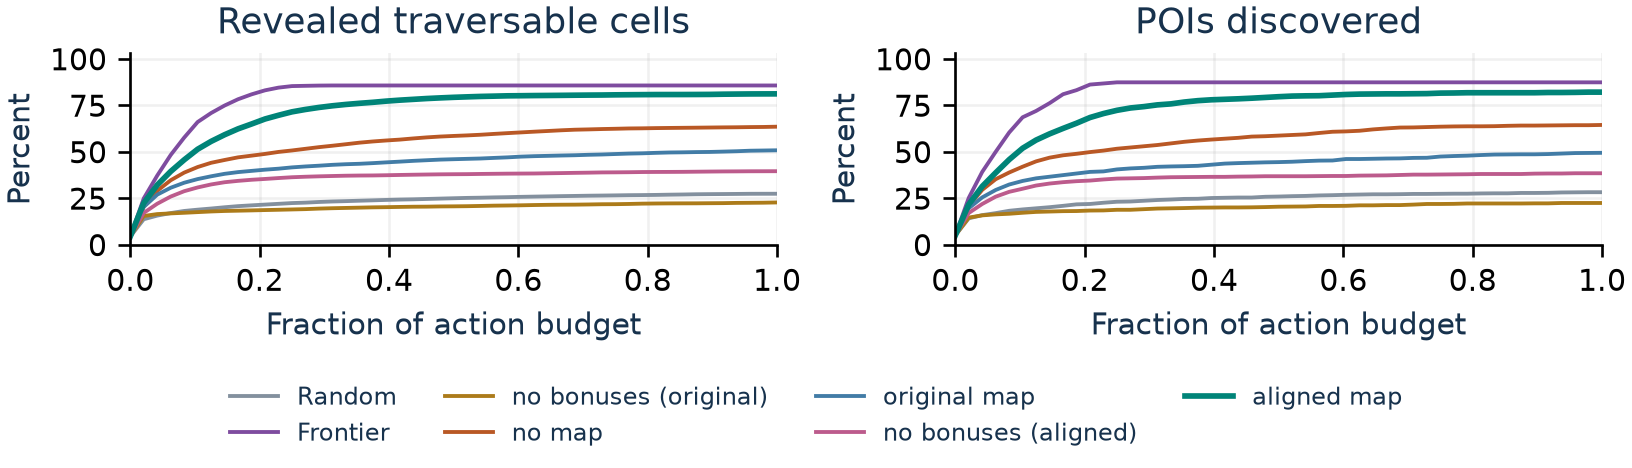
\includegraphics[width=\linewidth]{generated/hard-curves.png}
\caption{Hard coverage and discovery on reserved maps, retaining terminal values after death. The aligned no-bonus curve isolates reward removal with the aligned architecture held fixed.}
\label{fig:curves}
\end{figure}

\subheading{Generalization.} Medium-to-Hard coverage falls 12.4 pp aligned, versus 18.3 pp original, 15.3 pp mapless, and 7.0 pp frontier. Hard changes size, POIs, budget, and relative spatial extent jointly. Against an earlier 50-map training-partition diagnostic of the same full-reward models, aligned confirmation coverage differs by -0.5 / +1.6 / +0.1 pp (Easy/Medium/Hard); seed numbers do not guarantee training exposure, and no Hard maps were trained on. Comparable Easy/Medium confirmation AUC is 0.877 versus selected validation 0.883; the three-preset AUC of 0.825 also includes Hard.

\newpage
\heading{8\quad Failure cases}
The following historical, post-hoc examples are separate from the reserved confirmation set.

\subheading{Survival without exploration.} On Hard map 30029, aligned training seed 11 survives all 1,536 actions but reveals only 10.0\pct\ of terrain, discovers no POIs, and loops on 99.9\pct\ of actions. The map records history but does not ensure that the policy uses it to leave a familiar region. Survival alone would miss this failure.

\subheading{Early threat contact.} On Hard map 30002, the same run dies after 32 actions with 8.2\pct\ coverage and one POI. Clearing outdated threat positions avoids stale occupancy but leaves the agent without threat tracking under occlusion. Predictive threat history is a possible extension, rather than an established explanation for this contact.

On confirmation maps, aligned Hard loops affect 50.6\pct\ of actions, versus 32.5\pct\ mapless and 52.0\pct\ original. Some repeats occur after useful exploration is complete, so the coverage context matters. Wall contacts average 1.47\pct\ of all aligned actions versus 0.53\pct\ mapless; this is not an error rate per forward attempt. Higher exploration may increase threat exposure, but that causal link has not been isolated.

\heading{9\quad Computational feasibility and reproducibility}
Earlier isolated CPU timing of the same full-reward models uses one process/thread, two shared validation maps per preset, and 96 episodes. Action selection plus input preprocessing includes the first action but excludes physics, rendering, and loading. Aligned PPO averages 1.204 ms (p95 1.427), versus 0.884 ms original, 0.891 ms mapless, and 0.523 ms frontier. Alignment adds gathering work without parameters; the map encoder remains 70.6\pct\ of capacity. These measurements describe this machine and workload.

The \href{https://github.com/emkienngu123/MiniGridRL}{MiniGridRL repository} retains Farama history and Apache-2.0 attribution. Configurations, versioned/hashed checkpoints, raw measurements, training histories, and CPU/UI instructions support reproduction; aligned models are in \code{checkpoints/aligned/}. Checks cover determinism, information boundaries, rewards, geometry, and loading. The demo and Windows CPU build use validation-best aligned seed 33 (AUC 0.889863); historical artifacts remain archived separately.

\heading{10\quad Limitations and future work}
The comparison supports the aligned map readout and exploration bonuses within the tested generator, patrol rules, and training budget. It does not isolate every architectural choice: CNN widths, feature allocation, activations, encoder sharing, and visit-count saturation have no individual ablations. Reward weights, spawn separation, patrol intervals, and budgets are fixed engineering choices. Five million transitions and three seeds provide matched compute and replication, without establishing convergence or sufficient statistical power.

No DQN or recurrent-policy comparison establishes algorithm superiority. Reward scale and discounting may affect stalls and survival, but no sweep separates these effects. The no-map condition changes both information and effective capacity. The original rotation probes also modify heading and use out-of-distribution inputs; the retrained comparison is the primary evidence for alignment.

Useful next experiments would vary encoder size, visit saturation, reward/death balance, or discounting one at a time under the same validation protocol. Sampled-action evaluation and predictive or recurrent threat memory could address stalls and contact. More training seeds and independently reserved maps would broaden the evidence; the current confirmation maps are now observed. Hard remains a joint extrapolation test over scale and task settings.

\textbf{Conclusion.} Centering and rotating the observation-derived map made spatial history more useful to the same PPO network, improving coverage and discovery on reserved maps. Frontier explores faster, while PPO retains looping and survival failures. The resulting agent is an effective exploration policy within this setting, with clear limits in threat handling and generalization.

{\footnotesize
\setlength{\parskip}{1pt}
\bibliographystyle{abbrv}
\bibliography{references}
}
\end{document}
